\section{Controller}
\begin{figure}[H]	
	\centering
    \frame{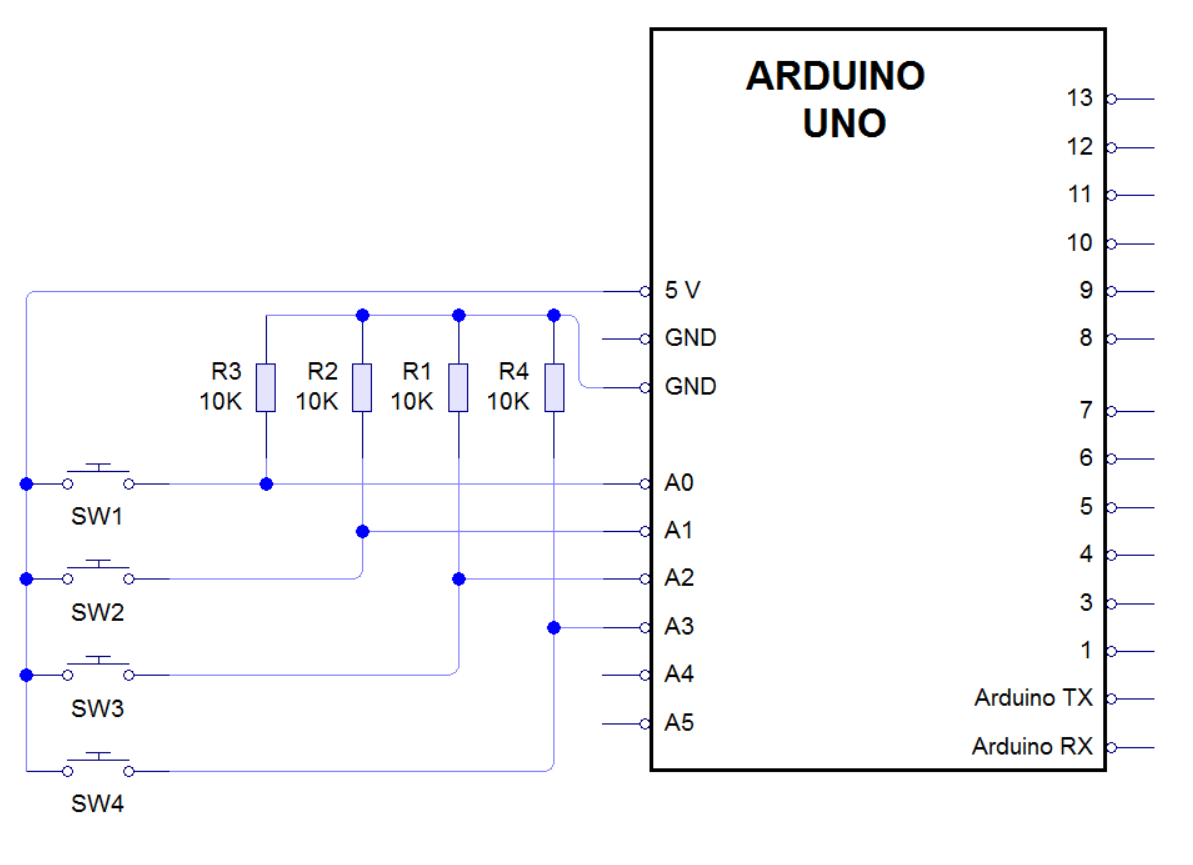
\includegraphics[width=10cm]{figures/2_4kredse/controller.png}}
	\caption{Et billede af kredsløbet for controller kredsen.}
	\label{kreds:controller}
\end{figure}

\subsection{Komponenter}
I kontrolleren bliver der kun brugt simple fysiske switches og modstande.

\subsection{Teori}
For at undgå en kortslutning bliver der sat en modstand imellem den ene switch side og ground. På den anden side a switchen er der $\SI{5}{V}$.
%\subsection{Beregninger}

%\subsection{Test}